% !TeX root = ../main.tex

\chapter{张量网络态}

\section{张量}

\subsection{张量的定义}

\subsubsection{抽象定义}

若$V_i$与$W_i$都是域$\mathbb{F}$上的有限线性空间,$\otimes$是张量积,那么一个张量即是原空间$W_i$与对偶空间$V^*_i$的张量积空间中的一个元素,若张量积空间由$p$个原空间与$q$个对偶空间构成,则其上张量被称为$(p,q)$阶的:
\[
\text{order-}(p,q) \text{ tensor } \symbf{T} \in W_1 \otimes W_2 \otimes \dots \otimes W_p 
\otimes V^*_1 \otimes V^*_2 \otimes \dots \otimes V^*_q
\]

若$\{{e^{(i)}}_k\}$与$\{{\eta^{(i)}}_k\}$分别为空间$W_i$与对偶空间$V^*_i$的基,则利用爱因斯坦求和约定,张量可以被表示为分量和的形式:
\[
\symbf{T}=T^{i_1\dots i_p}_{j_1\dots j_q} \,\, {e^{(1)}}_{i_1}\otimes\dots\otimes{e^{(p)}}_{i_p}
\otimes {\eta^{(1)j_1}}\otimes\dots\otimes{\eta^{(q)j_q}}
\]

用于描述量子多体系统的张量网络是由具体的张量表示的,因此为了更方便与准确的表示本文中的张量,我们将张量的定义特殊化以方便描述本文中使用的张量。

\subsubsection{具体定义}

一个实数域或复数域上的有限多维数组$\{T_{i_1 i_2\dots i_p}\}$被称为一个张量,若表示一个张量的数组的维度为$p$,则称此张量为$p$阶的。若第$k$个指标$i_k$的取值范围为集合$S_{k}$,则$\lvert S_{k}\rvert$称为指标$i_k$的维数。若两个同阶张量的指标维数依次相等,则称两个张量是相同形状的。

\begin{figure}[htb]
	\centering
	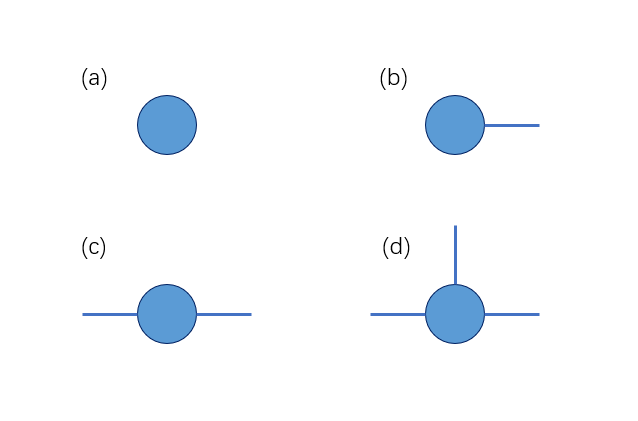
\includegraphics[width=1\textwidth]{image/Tensor.png}
	\caption{张量网络的图表示}
	\label{fig:sgd-svrg2}
	\note{注:(a)零阶张量,标量;(b)一阶张量,矢量;(c)二阶张量,矩阵;(d)三阶张量。}
\end{figure}

相较于上文中的定义,这里应用了以下改动:
\paragraph{指定数域}
一个量子系统至多在复数域即可被表示,因此这里把数域指定为实数域或复数域,此时张量可表示为实数或复数域上的多维数组。
\paragraph{约定形式}
本文中的张量有两种指标,一种是由实空间取向标记的缩并指标,一种是由对应的自旋分量(通常为$\hat{\symbf{S}}_z$的本征值)标记的物理指标。这里我们至多只需研究张量在不同自旋右矢下的变换,因此不严格区分协变与逆变指标,默认张量为$(0,p)$或$(p,0)$阶的。



\subsection{张量的运算}

\subsubsection{加法运算}

两个相同形状的张量$A$与$B$之间可以定义加法:$\symbf{C} = \symbf{A}+\symbf{B}$,即:
\begin{equation}
C_{i_1 i_2 \dots i_p} = A_{i_1 i_2 \dots i_p} + B_{i_1 i_2 \dots i_p}
\end{equation}


\subsubsection{数乘运算}

对任意$\alpha \in \mathbb{C}$,可定义张量与其的数乘运算:$\symbf{M}' = \alpha \symbf{M} = \symbf{M} \alpha$,即:
\begin{equation}
M_{i_1 i_2 \dots i_p}' = \alpha M_{i_1 i_2 \dots i_p}
\end{equation}

\subsubsection{缩并运算}
\begin{figure}[htb]
	\centering
	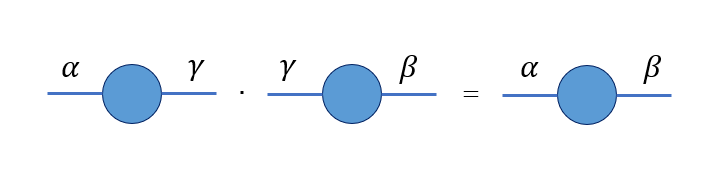
\includegraphics[width=1\textwidth]{image/TensorContr.png}
	\caption{张量缩并}
	\label{fig:contract}
	\note{注:相同指标$\gamma$缩并后消失,图示与矩阵乘法一致。}
\end{figure}

若两个张量$\symbf{A}$与$\symbf{B}$间的一个或者一些指标维数分别相同,则可以定义缩并运算对重复指标遍历求和:
\begin{equation}
C_{\alpha\beta} = \sum_{\gamma=1}^{D_\gamma} A_{\alpha\gamma} B_{\gamma\beta}
\end{equation}
或
\begin{equation}
C_{\alpha\beta} = \sum_{\delta,\gamma,\nu=1}^{D_\delta,D_\gamma,D_\nu} A_{\alpha\delta\gamma\nu} B_{\gamma\beta\nu\delta}
\end{equation}
所得张量的未缩并指标可继续缩并:
\begin{equation}
\label{eq.1.5}
M_{\alpha m n} = \sum_{\beta=1}^{D_\beta} C_{\alpha\beta} F_{\beta m n}
	= \sum_{\delta,\gamma,\nu,\beta=1}^{D_\delta,D_\gamma,D_\nu,D_\beta} A_{\alpha\delta\gamma\nu} B_{\gamma\beta\nu\delta} F_{\beta m n}
\end{equation}

\subsubsection{分解运算}

分解可看作缩并的逆运算。若给定张量$\left\{M_{\alpha m n}\right\}$,则如公式$(\ref{eq.1.5})$中将张量表示为几个张量的缩并的形式,称为张量的分解。

由以上定义易知,相同形状的张量构成线性空间,其加法与数乘的性质与矢量一致,且张量之间缩并的先后顺序不影响结果。下文中为了书写方便,声明求和约定后,张量缩并均采用爱因斯坦求和约定,即默认重复出现的指标需要求和。例如公式$(\ref{eq.1.5})$重新写为:
\[
M_{\alpha m n} = C_{\alpha\beta} F_{\beta m n}
	= A_{\alpha\delta\gamma\nu} B_{\gamma\beta\nu\delta} F_{\beta m n}
\]


\section{张量网络}

\subsection{张量网络的定义}

张量网络是一组张量的集合与其上的缩并规则构成的数学结构。整个张量网络等效于一个巨大的张量\cite{hsiaoJournalClubBrief}。

张量网络的全部结构由无向图$G=(V,E)$表示,其中顶点集$V$为空顶点集$V_L$与张量顶点$V_T$的不交并,边集$E$为$E_L$与$E_T$的不交并(指交集为空的两个集合的并集)。表示规则为:
\paragraph{每个张量与$V_T$中元素一一对应;}

\paragraph{每个未缩并指标与$V_L$,$E_L$中元素都一一对应;}

\paragraph{每对缩并指标与$E_T$中元素一一对应。}

边集$E$中元素被称为脚,$E_L$中元素只与一个张量顶点相连,我们称其为“悬空脚”,又因为其对应真实的自旋等有物理意义的量,所以也被称为物理脚;$E_T$中元素连接两个张量顶点,我们称其为“缩并脚”或者“键”。

\subsection{张量网络的图表示法}

每个张量网络都对应一个无向图,因此我们可以将图画出,通过图形来了解张量网络的结构。在通常的无向图上,我们将张量顶点扩大为空心图形着重显示,用以代表此顶点对应点的张量。这种无向图的表示被称为张量网络图。

在张量网络图中,每个$n$阶张量一定有$n$个脚,需要缩并的张量之间公共脚的个数对应需要缩并的指标个数,每个脚对应的指标的维数不表示在图中。相比于文字叙述或代数表达,张量网络图能够更直观的表示张量网络的结构,也使得我们能更高效的描述对网络施加的缩并、分解等操作。

\begin{figure}[htb]
	\centering
	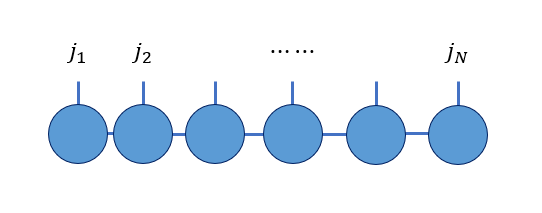
\includegraphics[width=1\textwidth]{image/smallTensors.png}
	\caption{张量网络之矩阵乘积态}
	\label{fig:MPS}
	%\note{}
\end{figure}

\subsection{张量网络的运算}

\subsubsection{张量网络的缩并}

一个张量网络中的张量之间存在缩并关系,当我们应用这些关系将某些张量缩并为一个张量时,其张量网络图中对应的边表现为收缩至消失,且其两端的张量顶点融合为一个,如图\ref{fig:contract}。这种操作被称之为张量网络对其边(键)的缩并。

\subsubsection{张量网络的分解}

如同张量的分解可看做张量缩并的逆运算,张量网络的分解也可借助其缩并来定义。当我们将网络中的某些张量分别拆分为其他张量的缩并时,这种操作被称之为张量的分解,如图\ref{fig:decp}所示。

\begin{figure}[htb]
	\centering
	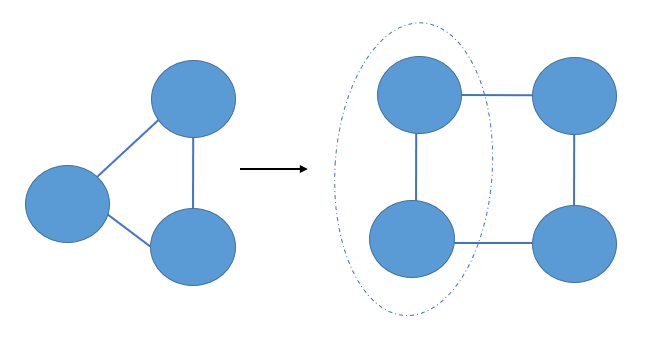
\includegraphics[width=0.8\textwidth]{image/decomposition.png}
	\caption{张量网络的分解}
	\label{fig:decp}
	%\note{}
\end{figure}

\section{张量网络与量子态}

\subsection{量子态的常规表示}

上文主要介绍了张量网络的相关定义以及性质,本节我们将说明张量网络具体应怎样应用至量子态的表示。

在从多体量子态过渡到张量网络之前,我们先回顾一下多体系统的一些概念。

\subsubsection{直积态}

两个量子系统的纯态分别记为$\ket{\phi_1}\in\mathcal{H}_1$与$\ket{\phi_2}\in\mathcal{H}_2$,纯态$\ket{\varphi}\in\mathcal{H}$表示两个量子系统视为一个整体时的量子态,则$\mathcal{H} = \mathcal{H}_1\otimes\mathcal{H}_2$. 若$\ket{\varphi}$具有形式
\begin{equation}\label{eq-product-state}
\ket{\varphi}=\ket{\phi_1}\otimes\ket{\phi_2}
\end{equation}
则$\ket{\varphi}$被称为直积态。否则,其被称为纠缠态。对于两体纠缠态,其不能直接写为两个纯态的直积,被表示为一系列直积之和
\begin{equation}\label{eq-product-state-sum}
\ket{\varphi} = \sum_{i,j}^{d_i,d_j} c_{i,j}\ket{i}\ket{j}
\end{equation}

为了研究这个两体系统的性质,我们可能会用到一些数学处理。

\subsubsection{奇异值分解}

对任意矩阵$\symbf{A}\in\mathbb{C}^{M\times N}$做奇异值分解\cite{stewartEarlyHistorySingular1993}(Singular Value Decomposition, SVD)得
\begin{equation}\label{eq-SVD}
\symbf{A} = \symbf{U} \Lambda \symbf{V}^\dagger
\end{equation}
(1) $\symbf{U}\in\mathbb{C}^{M\times L},\: \symbf{U}^\dagger \symbf{U}=\symbf{I}$;\\(2) $\symbf{V}^\dagger\in\mathbb{C}^{L\times N},\: \symbf{V}^\dagger \symbf{V}=\symbf{I}$;\\(3) $\symbf{\Lambda}$ 为$L\times L$非负实对角阵,对角元素$\lambda_i$称为奇异值,且非$0$对角元素个数称之为$A$的秩,对任意酉不变范数有$\lVert \symbf{A} \rVert^2=\sum_i \lambda_i^2$. 其中$L=\min(M,N)$.

\subsubsection{施密特分解}

对于有限维的两体纠缠系统,存在一种称为施密特分解的方法,它将(\ref{eq-product-state-sum})中的量子态分解为以下形式
\begin{equation}\label{eq-sd-phi}
\ket{\varphi}=\sum_{i=1}^{\chi} \lambda_i \ket{i_A}\ket{i_B}
\end{equation}
其中$\lambda_i$为正数且有$\sum_i \lambda_i^2 = 1$. 施密特分解可由奇异值分解得来,我们只需将SVD分解应用在$\{c_{i,j}\}$上,
\begin{align}
	\ket{\varphi} &= \sum_{i,j}^{d_i,d_j} c_{i,j}\ket{i}\ket{j} \\
		 &= \sum_{i,j}^{d_i,d_j} \sum_k^\chi u_{i,k} \lambda_{k} v_{k,j} \ket{i}\ket{j}\\
		 &= \sum_k^\chi \lambda_k \left( \sum_i^{d_i}u_{i,k}\ket{i} \right) \left( \sum_j^{d_j}v_{k,j}\ket{j} \right)\\
		 &= \sum_{k=1}^{\chi} \lambda_k \ket{k_A}\ket{k_B}\\
		 &= \sum_{i=1}^{\chi} \lambda_i \ket{i_A}\ket{i_B}
\end{align}
矩阵$\left\{c_{i,j}\right\}$的秩$\chi$在这里被称为施密特秩,被某一表象下的$\ket{\varphi}$唯一确定。施密特秩可以用来衡量两体系统之间纠缠状态数的多少,也经常会出现在对多体系统的分析中。

\subsubsection{纠缠熵}

在零温时,纯态量子系统的冯诺依曼熵为零,但选取一部分子系统单独查看,其熵可能不为零。这部分仅仅由量子系统的纠缠产生的熵被定义为冯诺依曼纠缠熵\cite{eisertColloquiumAreaLaws2010}
\begin{equation}
\mathcal{S}(\symbf{\rho}_A) = -\Tr(\symbf{\rho}_A\log\symbf{\rho}_A) = -\Tr(\symbf{\rho}_B\log\symbf{\rho}_B)
\end{equation}
其中$A,B$是系统一分为二的两部分,$\rho_A$是密度矩阵对$B$系统求部分迹得到的约化密度矩阵,反之同理。若利用施密特分解将系统$\ket\varphi$分为(\ref{eq-sd-phi})中的两部分,则冯诺依曼纠缠熵可以表达为
\begin{equation}
\mathcal{S} = -\sum_i^\chi \lambda_i^2\log\left(\lambda_i^2\right)
\end{equation}

纠缠熵是一个用来衡量量子系统纠缠大小的物理量。一个具有纠缠的基态的强关联系统有时能表现出特殊的集体量子行为\cite{vidalEntanglementQuantumCritical2003},因此纠缠熵在研究强关联系统时有重要意义。通常情况下,基态附近的量子态均满足纠缠熵面积定律,$d$维系统的纠缠熵正比于边界面积$L^{d-1}$. 
\subsubsection{多体系统}
通常情况下,我们会遇到由$N$粒子构成的量子多体系统,其每一个粒子具有维度为$p$的态空间。最常见的例子即是一个由自旋$\frac12$的粒子组成的$N$粒子自旋系统,其$p=2$. 要表示这样的量子态,我们可以选择单体$\hat{\symbf{S}}_z$算符的本征态$\ket{j_k}$为每个粒子态空间的基,这样整体态空间的基可由每个粒子态空间基的直积构成,整体的态矢$\ket{\varphi}\in\left(\mathbb{C^d}\right)^{\otimes N}$表示为
\begin{equation}\label{eq-1.6}
\ket{\varphi} = \sum_{j_1 \dots j_N} c_{j_i \dots j_N}\ket{j_1 \dots j_N}
	= \sum_{j_1 \dots j_N}c_{j_i \dots j_N}\ket{j_1}\otimes \dots \otimes\ket{j_N}
\end{equation}
其中$j_k=\,\uparrow\text{或 }\downarrow$. 系数$c_{j_i \dots j_N}\in\mathbb{C}$对于所有的指标构成一个张量 $\left\{c_{j_i \dots j_N}\right\}$,将其用张量网络图表示如图\ref{fig:bigTensor}。在这种表示中,表示一个$N$体系统的量子态需要的参数的个数为$2^N$,它随系统规模的增大而指数级增大。若想利用计算机来计算这个多体系统的有关性质,所需程序的空间复杂度至少是$\mathcal{O}\left(2^N\right)$的。在这种情况下,程序可计算的系统大小就会因为内存间有限等原因被限制在很小的规模。

\begin{figure}[htb]
	\centering
	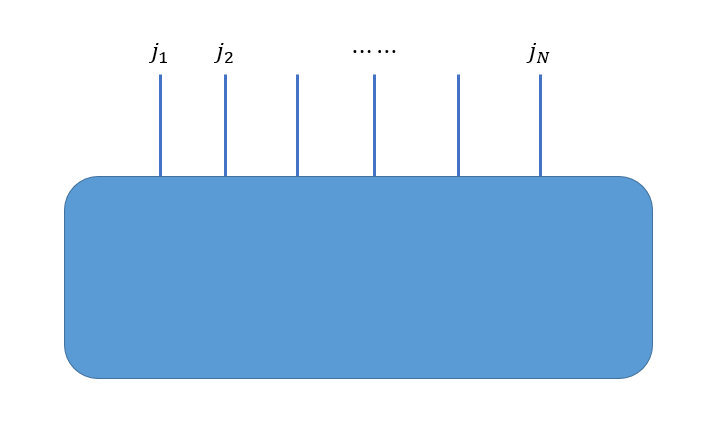
\includegraphics[width=1\textwidth]{image/bigTensor.png}
	\caption{系数矩阵看做张量}
	\label{fig:bigTensor}
	%\note{}
\end{figure}

为了解决这个问题,我们希望寻找上述系统的其它的表示方式。这种表示方式应该避免指数级的空间复杂度,并且能正确的表示系统的状态。

\subsection{矩阵乘积态}
\subsubsection{描述}

为了避免过高的空间复杂度,一种可行的方法是将整个张量拆分为不同的小张量的缩并。其中被构造出的一种一维结构叫做矩阵乘积态(Matrix Product State, MPS),它在周期边界条件下将$\ket{\varphi}$表示为
\begin{equation}\label{MPS_PBC}
\ket{\varphi} = \sum_{j_1\dots j_N}^p \Tr\left( \symbf{A}_{1}^{j_1} \symbf{A}_{2}^{j_2}\dots \symbf{A}_{N}^{j_N} \right)\ket{j_1 j_2\dots j_N}
\end{equation}
在开边界下表示为
\begin{equation}
\ket{\varphi} = \sum_{j_1\dots j_N}^p \bra{l} \symbf{A}_{1}^{j_1} \symbf{A}_{2}^{j_2}\dots \symbf{A}_{N}^{j_N}\ket{r} \:
\ket{j_1 j_2\dots j_N}
\end{equation}
上式中$\symbf{A}_n^{j_n}$表示第$n$个张量上自旋$j_n$对应的矩阵(2阶张量)。在周期边界条件下,考虑上文描述的$N$粒子$p$自旋系统,表示其量子态需要$\mathcal{O}\left(2^N\right)$的空间复杂度。公式(\ref{MPS_PBC})中需要的参数个数为小矩阵的和,系统中每个粒子的每个状态对应一个参数矩阵,因此整体的空间复杂度为$\mathcal{O}(NpD^2)$,其中$D$来自于假设每个矩阵$\symbf{A}_{n}^{j_n}\in \mathbb{C}^{D\times D}$. 在新的表示方式下,系统的空间复杂度降低为多项式级,这样在系统规模不断扩大时,我们计算所需的空间开销增速显著减慢,这意味着我们可以承受对更大规模系统的计算。
\begin{figure}[htb]
	\centering
	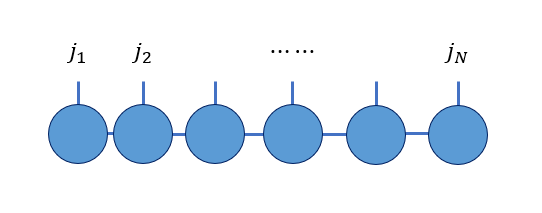
\includegraphics[width=1\textwidth]{image/smallTensors.png}
	\caption{开边界条件的MPS}
	\label{fig:MPS-OBC}
	%\note{}
\end{figure}
\begin{figure}[htb]
	\centering
	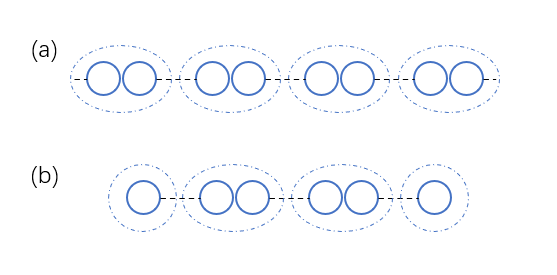
\includegraphics[width=1\textwidth]{image/VBS_o_and_p.png}
	\caption{VBS态}
	\label{fig:VBS}
	\note{(a)周期边界条件下的VBS态;(b)开边界条件下的VBS态。同一虚线圈中的对象对应真实空间同一个格点}
\end{figure}
\subsubsection{VBS态}
另一种定义MPS的方式是通过 Valance Bond States \cite[8]{dongZhangLiangWangLuoSuanFaCongBoSeZiXiTongDaoFeiMiZiXiTong2017}来构造系统的量子态。我们考虑上文中一维周期边界条件上的自旋链,每个格点上由两个相同的自由度为$D$的粒子$a_i$与$b_i$,每个粒子与相邻格点形成最大纠缠态
\begin{equation}
\ket{\varphi(b_i a_{i+1})} = \ket{I} = \sum_{\alpha=1}^D \ket{\alpha,\alpha},
\end{equation}
整个系统由
\begin{equation}
\ket{\varPhi} = \ket{I}^{\otimes N}
\end{equation}
构成,如图\ref{fig:VBS}(a)。每一对粒子$a_i,b_i$构成比原先单粒子空间更大的希尔伯特空间。在构造完成后,我们需要将非物理的自由度排除,使其回到原先的空间,因此在第$n$个格点考虑我们需要用到的投影算符$\hat{\symbf{A}}(n)$
\begin{equation}
\hat{\symbf{A}}(n) = \sum_{i=1}^p\sum_{\alpha,\beta=1}^D {A}(n)^i_{\alpha,\beta}\ket{i}\bra{\alpha,\beta}
\end{equation}
将其逐点作用在$\ket\varPhi$上\cite[16]{bridgemanHandwavingInterpretiveDance2017},我们便得到了与(\ref{MPS_PBC})相同的量子态$\ket\varphi$。公式中出现的$A(n)^i_{\alpha,\beta}$正是张量网络中出现的张量$\symbf{A}_n$的各个分量。这里使用的边界条件为周期边界条件,对于开边界条件也可类似地构造,如图\ref{fig:VBS}(b).
\subsubsection{性质}

\paragraph{边界条件}

开边界条件下,MPS不具有平移对称性,因为原则上它的每个张量都可以是不同的。在周期边界条件下,我们将系统由指定的元胞无限平移而成,那么对应的张量网络也看做由指定张量序列无限平移形成的极限,它可以具有我们所表示系统的平移对称性。

\paragraph{纠缠熵面积定律}

纠缠熵面积定律指出,张量网络子系统的纠缠熵仅仅与子系统边界有关。MPS遵守纠缠熵面积定律,由于是一维系统,其边界是零维的端点,因此其边界与系统规模无关,纠缠熵$\mathcal{S}(L)=-\Tr\left(\symbf{\rho}_L\log\symbf{\rho}_L\right)=\mathcal{O}(\log\! D)$为常数\cite{PracticalIntroductionTensor2014},其中$\symbf{\rho}_L$为子系统$L$的约化密度矩阵。

纠缠熵面积定律是张量网络能够有效表示量子态的原理所在。对于有能隙的系统,其基态总是遵守纠缠熵面积定律,而任何遵守纠缠熵面积定律的量子态都能被MPS所表示\cite{eisertEntanglementTensorNetwork2013}。这就解释了为何MPS可以用更少的参数表示量子态:当我们关注系统在基态附近的性质时,系统所处的量子态只能是那些遵循纠缠熵面积定律的量子态,这些态都可以被MPS表示,系统的参数在面积定律的约束下大大减少。

\paragraph{关联长度有限}

两体关联反应一个算符在不同位置处时其期望值的相关程度
\begin{equation}
C(r) = \langle O_i O'_{i+r}\rangle - \langle O_i\rangle\langle O'_{i+r}\rangle
\end{equation}
在文献~\inlinecite{PracticalIntroductionTensor2014}的130页中给出了一个简单的例子,证明了一个长度为一的在MPS周期边界条件下关联函数是指数下降的。这种指数下降在一维有能隙系统中普遍存在,这侧面反映了为何MPS能很好的表示这种系统。反之,对处于相变点附近的,具有趋于无穷的关联长度的系统,MPS无法表示。

\paragraph{精确缩并复杂度}

计算两个MPS态的内积,即缩并两个MPS,其时间复杂度总可以达到$\mathcal{O}(NpD^3)$. 这个性质不难理解,因为我们的计算难度与计算$N$个矩阵的乘积并无本质区别。正是如此,我们的MPS算法可以高效运行,或者说不同于时间复杂度指数增加的算法,MPS上的算法复杂度计算大系统是可接受的。

\subsection{投影纠缠态}
\subsubsection{描述}

矩阵直积态利用多体系统基态的特点对多体系统的整个希尔伯特空间做了近似,并因此能够高效的描述一维多体系统。将这种方法推广到二维系统的一个尝试便是投影纠缠态(Projected Entangled Pair States, PEPS),它是许多二维格点算法的基础。同上文中矩阵乘积态的思想一致,我们希望将(\ref{eq-1.6})中系数构成的张量分解为小张量的缩并来减少参数。若我们的系统是一个$N\times M$的方形格点,我们可以按与系统格点相同的方式分解张量
\begin{equation}\label{PEPS_PBC}
\ket{\varphi} = \sum_{\{j\}} \Tr\left[ \symbf{A}{(1,1)}^{j_{1,1}} \symbf{A}{(1,2)}^{j_{1,2}}\dots \symbf{A}{(N,M)}^{j_{N,M}} \right]\ket{j_{1,1} j_{1,2}\dots j_{N,M}}
\end{equation}
这里的每个$\symbf{A}{(n,m)}^{j_{n,m}}$都是一个$4$阶张量,含有四个与周围张量缩并的键,整体上每个格点对应一个$5$阶张量$\symbf{A}{(n,m)} = A_{n,m}(l,r,u,d,j_{n,m})$,只有一个悬空脚为$j_{nm}$.

\begin{figure}[htb]
	\centering
	\includegraphics[width=1\textwidth]{image/PEPS1.png}
	\caption{开边界条件的MPS}
	\label{fig:PEPS}
	\note{注:图片引用自实验室师兄的文章\cite[31]{ErWeiLiangZiDuoTiXiTongDeZhangLiangWangLuoTaiSuanFaZhongGuoBoShiXueWeiLunWenQuanWenShuJuKu}. (a)键的维度为$D$的PEPS的图表示;(b)左矢和对应右矢构成的双层张量网络;(c)先对每个格点物理指标进行求和;(d)由c中$D^2\times D^2\times D^2\times D^2$的张量构成的张量网络。}
\end{figure}

\subsubsection{VBS态}

另外还有一种看待投影纠缠态的方式,是像上文中MPS那样将PEPS看做由高维希尔伯特空间中最大纠缠态投影得到的VBS态。我们考虑在系统的每个格点上共有4个虚拟的自由度为$D$的粒子分别与上下左右的格点中的相邻粒子成键,如图\ref{fig:VBS4}. 类似的构造
\begin{equation}
\symbf{A}(n,m) = \sum_{i=1}^p\sum_{l,r,u,d=1}^D {A(n,m)}^i_{l,r,u,d}\ket{i}\bra{l,r,u,d}
\end{equation}
便可得到(\ref{PEPS_PBC})中的结果

\begin{figure}[htb]
	\centering
	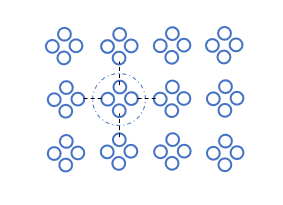
\includegraphics[width=0.8\textwidth]{image/VBS4.png}
	\caption{二维VBS态单格点示意}
	\label{fig:VBS4}
	%\note{注:图片来自实验室师兄的文章\cite[31]{ErWeiLiangZiDuoTiXiTongDeZhangLiangWangLuoTaiSuanFaZhongGuoBoShiXueWeiLunWenQuanWenShuJuKu}. (a)键的维度为$D$的PEPS的图表示;(b)左矢和右矢构成的双层张量网络;(c)先对每个格点物理指标进行求和;(d)由c中$D^2\times D^2\times D^2\times D^2$的张量构成的张量网络。}
\end{figure}

\subsubsection{性质}

\paragraph{边界条件}

对于开边界条件的PEPS,每个张量都可以是不同的,无平移对称性。对于周期边界条件的PEPS,我们的系统被看做由我们适当选择的元胞无限平移而成的2维晶格,因此张量网络对于任意格矢的平移都是对称的,它实际上表示了系统趋于无穷大时的极限状态。另外由于PEPS是2维的,我们可以选择某个方向为周期边界条件而另一个方向为开边界条件\cite[3]{osorioireguiInfiniteMatrixProduct2017},其图表示类似于圆柱体,这里不再展开说明。

\paragraph{纠缠熵面积定律}

纠缠熵面积定律适用于张量网络,但PEPS中的纠缠熵面积定律为2维形式,即任意子系统的纠缠熵正比于分割子系统的周长。若一个子系统的边界长为$L$,那么纠缠熵$\mathcal{S}(L)=\mathcal{O}(L\log\!D)$,其中$D$为上文中设置的键的维度,也可理解为VBS中设置的相邻系统之间的纠缠程度。

同MPS一样,PEPS的纠缠熵面积定律保证了其有能力表示有能隙系统的基态以及低能激发态。

\paragraph{关联函数多项式衰减}

PEPS与MPS之间一个很大的不同便是PEPS中两点之间的关联是随距离多项式衰减的,而上文的MPS是指数衰减的。仅仅这一项不同就使得PEPS具有了MPS不同的性质:从原理上来说PEPS不仅可以描述有能隙态,还可以描述临界态。呈多项式衰减的关联是临界系统的一大特征,因为临界系统具有标度不变性,其关联长度可以趋于无穷大\cite[138]{PracticalIntroductionTensor2014}。上文所说的MPS无法描述临界系统便是因为其关联长度永远是有限的,无法具有临界系统的特征。

\paragraph{精确缩并复杂度}

不论我们用什么顺序计算两个PEPS之间的缩并,其时间复杂度均是$\mathcal{O}\left(\exp(N)\right)$的\cite[139]{PracticalIntroductionTensor2014}。这一论断可被数学精确证明,它告诉我们尝试计算两个PEPS之间的缩并是低效的,对大系统来说更是不现实的。目前计算PEPS多采用近似算法,例如边界MPO近似\cite{lubaschUnifyingProjectedEntangled2014}等。

